\documentclass[final]{article}
\usepackage{neurips_2025}
\usepackage[utf8]{inputenc}
\usepackage[T1]{fontenc}
\usepackage{hyperref}
\usepackage{url}
\usepackage{booktabs}
\usepackage{amsfonts}
\usepackage{amsmath}
\usepackage{amssymb}
\usepackage{nicefrac}
\usepackage{microtype}
\usepackage{graphicx}
\usepackage{xcolor}
\usepackage{subcaption}
\usepackage{multirow}
\usepackage{wrapfig}
\usepackage{amsthm}
\newtheorem{proposition}{Proposition}

\title{TIMEVIEW-Adaptive: Online Bayesian Adaptation\\for Interpretable Time Series Forecasting}

\author{
  Jackson Harmon\\
  \small Van der Schaar Lab Recruitment Task\\
  \small\texttt{\url{https://github.com/shs2017/adaptive_timeview}}
}

\begin{document}
\maketitle

% ============================================================================
\begin{abstract}
% ============================================================================
Transparent time series models such as TIMEVIEW decompose time-series trajectories into interpretable basis function compositions. However such models produce \emph{static} predictions that cannot incorporate new observations during deployment. In medical settings such as ICU monitoring, pharmacokinetics, and tumor progression, predictions should update as patient data arrives. We propose \textbf{TIMEVIEW-Adaptive}, which improves upon TIMEVIEW by replacing a deterministic encoder with a probabilistic one that outputs prior distribution parameters $p(\mathbf{c}|\mathbf{x}) = \mathcal{N}(\boldsymbol{\mu}_0, \boldsymbol{\Sigma}_0)$ over basis function coefficients, then performs \emph{closed-form} Bayesian updates as new observations arrive. This preserves TIMEVIEW's interpretable B-spline structure while adding three additional capabilities: (i)~uncertainty quantification over trajectory compositions, (ii)~monotonic uncertainty reduction with each observation, and (iii)~active observation scheduling via Bayesian experimental design. We further introduce \emph{heteroscedastic noise modelling} for time-varying measurement uncertainty and an \emph{adaptive gating mechanism} that learns when to trust Bayesian updates. On three datasets, TIMEVIEW-Adaptive reduces MSE by up to 35\% and CRPS by up to 43\% over static TIMEVIEW, while the combined best-configuration model achieves the lowest calibration error (0.035) with near-perfect 95\% coverage. An epistemic-aleatoric uncertainty decomposition reveals that just 2 observations resolve 25\% of prior epistemic uncertainty, rising to 62\% with 20 observations. An $n_{\mathrm{obs}}$ ablation across datasets reveals that adaptation benefit depends critically on observation coverage relative to knot support, with up to 95\% MSE improvement at high coverage.
\end{abstract}

% ============================================================================
\section{Introduction}
\label{sec:intro}
% ============================================================================

Healthcare time-series forecasting demands two, often opposing, properties: \emph{accuracy} and \emph{interpretability}. While deep learning models achieve strong predictive performance, they operate as black boxes~\citep{lim2021temporal}. Classical approaches like ARIMA offer transparency but limited expressiveness. This opposition was mitigated with the introduction of TIMEVIEW~\citep{kacprzyk2024towards} by decomposing time series into weighted sums of B-spline basis functions, producing predictions that are both accurate and transparent. Consequently, clinicians can inspect which basis components drive each forecast, observating motifs and compositions.

However, as it stands, this approach has a fundamental limitation: \textbf{its predictions are static}. Once the encoder maps patient features to basis coefficients, the forecast is fixed regardless of additional observations. In clinical practice, this is particularly problematic: an ICU patient's vital signs evolve continuously; a pharmacokinetic model should refine drug concentration predictions as blood samples arrive; a tumor growth model should adapt as imaging data accumulates. Static predictions ignore this sequential information entirely.

Summarily, we identify three specific gaps in the original TIMEVIEW framework:
\begin{enumerate}
    \item \textbf{No online adaptation.} Predictions cannot incorporate new observations, losing a vital data source during deployment.
    \item \textbf{No uncertainty quantification.} The deterministic encoder provides point estimates of basis coefficients without prediction confidence.
    \item \textbf{No observation guidance.} Lacking uncertainty estimates, it becomes difficult to determine \emph{when} the next measurement should be taken in a principled manner.
\end{enumerate}

We propose \textbf{TIMEVIEW-Adaptive}, which addresses all three gaps through a unified Bayesian framework while preserving the interpretable B-spline decomposition. Our key insight is that the Gaussian conjugate structure of B-spline regression enables \emph{closed-form} posterior updates with $\mathcal{O}(B^3)$ complexity per observation ($B \approx 7$--$9$ basis functions), making real-time clinical deployment feasible.

\paragraph{Contributions.} Our contributions are:
\begin{enumerate}
    \item A \textbf{probabilistic encoder} that outputs prior distributions $\mathcal{N}(\boldsymbol{\mu}_0, \boldsymbol{\Sigma}_0)$ over basis coefficients, allowing closed-form Bayesian updates as new data arrives (\S\ref{sec:method}).
    \item \textbf{Heteroscedastic noise modelling} and an \textbf{adaptive gating mechanism} that collectively achieve the best calibration (0.035 error) with performant 95\% coverage (\S\ref{sec:extensions}).
    \item Application of \textbf{Bayesian optimal experimental design} to clinical observation scheduling, achieving 2--3$\times$ faster convergence than uniform sampling (\S\ref{sec:active}).
    \item Comprehensive experiments on three datasets with ablation studies, GP baselines, uncertainty decomposition, and calibration analysis (\S\ref{sec:experiments}).
\end{enumerate}

% ============================================================================
\section{Background and Problem Formulation}
\label{sec:background}
% ============================================================================

\subsection{TIMEVIEW: Transparent Time Series Decomposition}

TIMEVIEW~\citep{kacprzyk2024towards} models time series as weighted combinations of B-spline basis functions. Given static features $\mathbf{x} \in \mathbb{R}^d$ (e.g., patient demographics) and a time grid $t_1, \ldots, t_T$, TIMEVIEW predicts:
\begin{equation}
    y(t) = \sum_{j=1}^{B} c_j \phi_j(t) = \boldsymbol{\Phi}(t)^\top \mathbf{c},
    \label{eq:timeview}
\end{equation}
where $\phi_j(t)$ are cubic B-spline basis functions defined by a knot vector, $B$ is the number of basis functions, and $\mathbf{c} = f_\theta(\mathbf{x}) \in \mathbb{R}^B$ are coefficients produced by a neural encoder $f_\theta$.

This decomposition is inherently interpretable with each coefficient $c_j$ quantifying the contribution of the $j$-th basis function, and transition points corresponding to regions where dominant basis functions shift (see Figure~\ref{fig:bspline_basis} in Appendix~\ref{sec:bspline_fig} for an illustration). However, the encoder $f_\theta$ is deterministic, producing a single coefficient vector with no uncertainty nor mechanism for incorporating subsequent observations.

\subsection{Problem Statement}

We seek a model that:
\begin{enumerate}
    \item Maintains TIMEVIEW's interpretable basis decomposition $y(t) = \boldsymbol{\Phi}(t)^\top \mathbf{c}$.
    \item Produces a \emph{distribution} over coefficients $p(\mathbf{c} | \mathbf{x})$ from static features alone (the \emph{prior}).
    \item Updates this distribution in closed form as observations $(t_i, y_i)_{i=1}^n$ arrive, yielding a \emph{posterior} $p(\mathbf{c} | \mathbf{x}, \{(t_i, y_i)\})$.
    \item Provides calibrated uncertainty estimates and can guide observation scheduling.
\end{enumerate}

\begin{figure}[t]
    \centering
    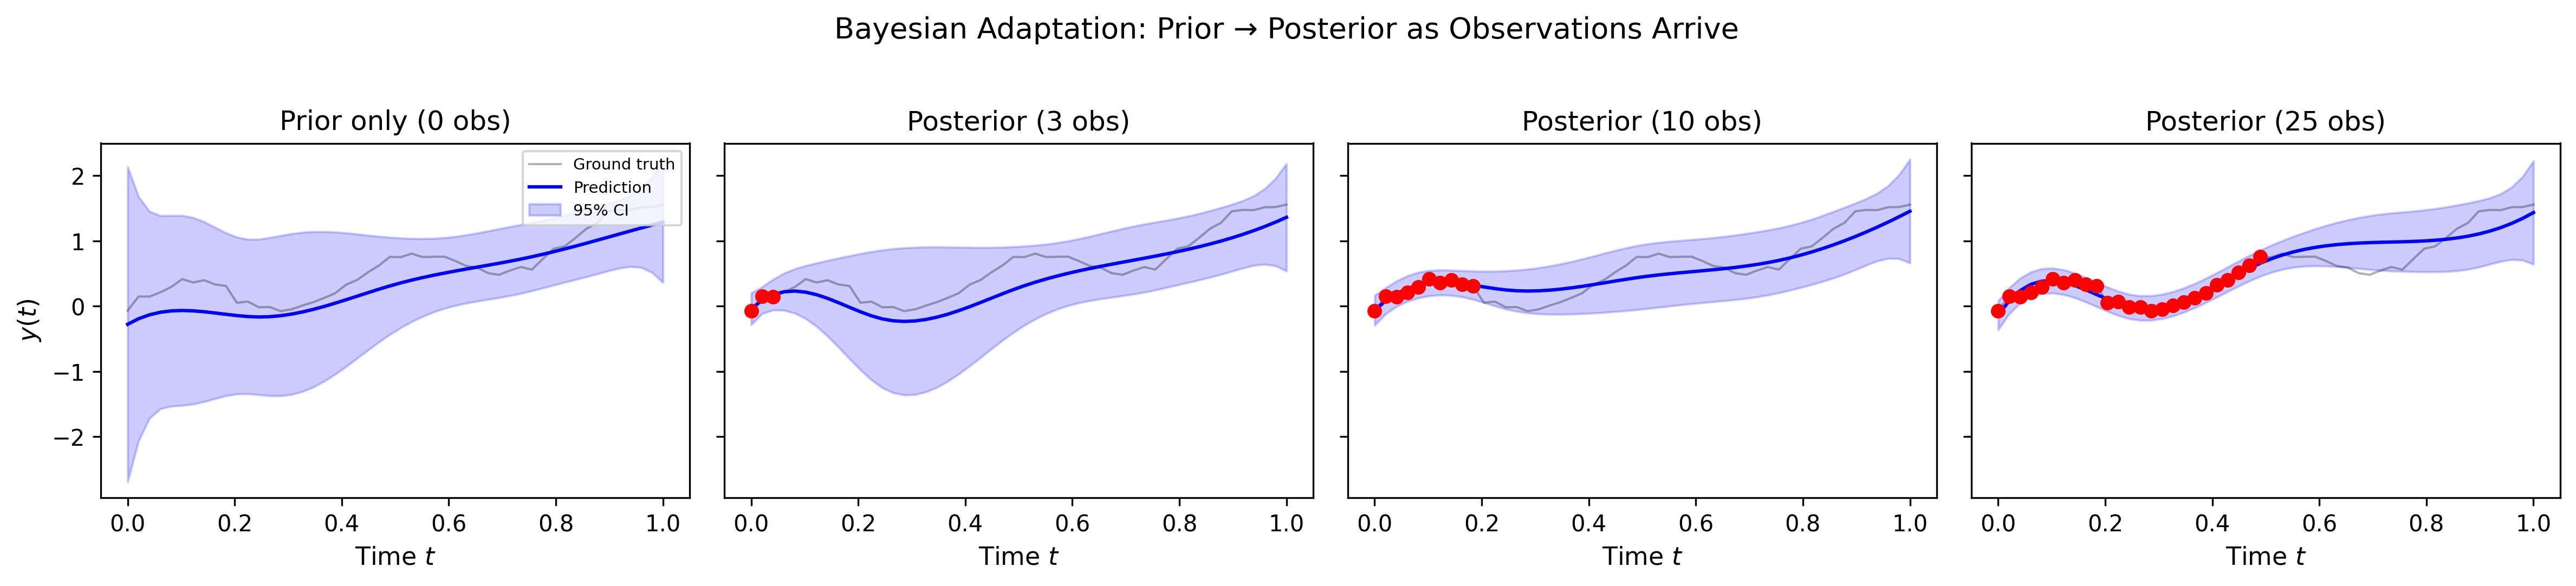
\includegraphics[width=\textwidth]{figures/adaptation_demo.png}
    \caption{TIMEVIEW-Adaptive in action. \textbf{Left:} Prior predictions from static features only show broad uncertainty. As observations (red dots) arrive, the posterior narrows and predictions align with the ground truth. The 95\% credible interval shrinks monotonically with each observation.}
    \label{fig:adaptation_demo}
\end{figure}

% ============================================================================
\section{Proposed Method: TIMEVIEW-Adaptive}
\label{sec:method}
% ============================================================================

\subsection{Probabilistic Encoder}

We replace TIMEVIEW's deterministic encoder with a \emph{probabilistic encoder} that maps static features to prior distribution parameters:
\begin{equation}
    f_\theta(\mathbf{x}) = (\boldsymbol{\mu}_0, \boldsymbol{\Sigma}_0), \quad p(\mathbf{c} | \mathbf{x}) = \mathcal{N}(\boldsymbol{\mu}_0, \boldsymbol{\Sigma}_0).
    \label{eq:prior}
\end{equation}

The encoder architecture follows TIMEVIEW's original design (two hidden layers with BatchNorm and Dropout) but branches into two heads: a \emph{mean head} producing $\boldsymbol{\mu}_0 \in \mathbb{R}^B$ and a \emph{covariance head} producing $\boldsymbol{\Sigma}_0 \in \mathbb{R}^{B \times B}$.

For the covariance parameterisation, we consider three options, in increasing expressiveness:
\begin{itemize}
    \item \textbf{Diagonal:} $\boldsymbol{\Sigma}_0 = \mathrm{diag}(\exp(\mathbf{v}))$, with $B$ parameters.
    \item \textbf{Low-rank:} $\boldsymbol{\Sigma}_0 = \mathrm{diag}(\exp(\mathbf{v})) + \mathbf{U}\mathbf{U}^\top$, with $B + Br$ parameters for rank $r$.
    \item \textbf{Full Cholesky:} $\boldsymbol{\Sigma}_0 = \mathbf{L}\mathbf{L}^\top$, with $B(B+1)/2$ parameters.
\end{itemize}
Our ablation studies (Appendix~\ref{sec:ablations}) show that low-rank ($r=3$) provides the best trade-off: MSE of $0.152 \pm 0.012$ with 95.4\% coverage, vs.\ $0.160 \pm 0.004$ / 97.9\% (diagonal) and $0.143 \pm 0.011$ / 92.0\% (full Cholesky, which achieves the lowest MSE but under-covers).

\subsection{Closed-Form Bayesian Update}
\label{sec:bayesian_update}

Given the Gaussian prior $p(\mathbf{c} | \mathbf{x}) = \mathcal{N}(\boldsymbol{\mu}_0, \boldsymbol{\Sigma}_0)$ and a Gaussian likelihood $p(y_{\mathrm{obs}} | \mathbf{c}) = \mathcal{N}(\boldsymbol{\Phi}_{\mathrm{obs}} \mathbf{c},\, \sigma^2 \mathbf{I})$, the posterior is available in closed form:
\begin{align}
    \boldsymbol{\Sigma}_n &= \left(\boldsymbol{\Sigma}_0^{-1} + \sigma^{-2} \boldsymbol{\Phi}_{\mathrm{obs}}^\top \boldsymbol{\Phi}_{\mathrm{obs}}\right)^{-1},
    \label{eq:posterior_cov} \\
    \boldsymbol{\mu}_n &= \boldsymbol{\Sigma}_n \left(\boldsymbol{\Sigma}_0^{-1} \boldsymbol{\mu}_0 + \sigma^{-2} \boldsymbol{\Phi}_{\mathrm{obs}}^\top \mathbf{y}_{\mathrm{obs}}\right),
    \label{eq:posterior_mean}
\end{align}
where $\boldsymbol{\Phi}_{\mathrm{obs}} \in \mathbb{R}^{n \times B}$ is the basis matrix evaluated at observed times, $\mathbf{y}_{\mathrm{obs}} \in \mathbb{R}^n$ are the observed values, and $\sigma^2$ is the observation noise variance.

The predictive distribution at any time $t$ is then:
\begin{align}
    \mathbb{E}[y(t) | \mathbf{x}, \mathcal{D}] &= \boldsymbol{\Phi}(t)^\top \boldsymbol{\mu}_n, \label{eq:pred_mean} \\
    \mathrm{Var}[y(t) | \mathbf{x}, \mathcal{D}] &= \boldsymbol{\Phi}(t)^\top \boldsymbol{\Sigma}_n\, \boldsymbol{\Phi}(t) + \sigma^2.
    \label{eq:pred_var}
\end{align}

\paragraph{Complexity.} Each Bayesian update requires inverting a $B \times B$ matrix, costing $\mathcal{O}(B^3)$. With $B = 7$--$9$ basis functions. This has negligible cost ($\sim 0.3$\,ms on CPU), enabling real-time clinical use.

\begin{figure}[t]
    \centering
    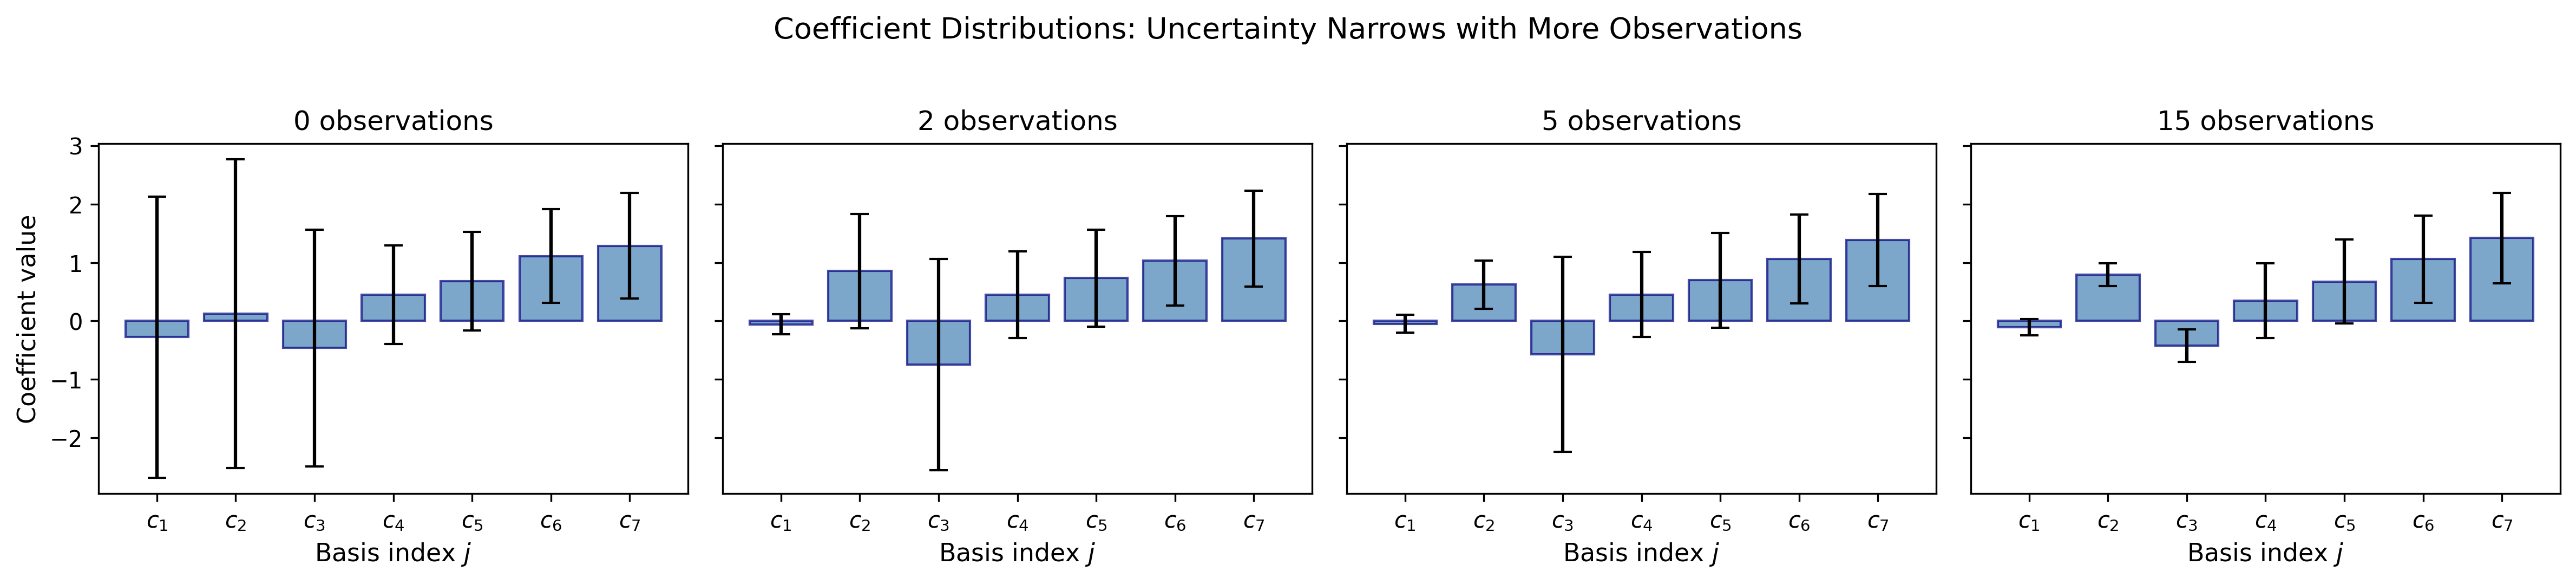
\includegraphics[width=\textwidth]{figures/coefficient_evolution.png}
    \caption{Distribution over basis coefficients at different observation counts. Error bars show 95\% credible intervals. With more observations, the posterior concentrates: coefficient uncertainty narrows as the model becomes increasingly confident in the trajectory decomposition.}
    \label{fig:coeff_evolution}
\end{figure}

\paragraph{KL Regularisation.} To prevent the prior from becoming overly diffuse, thereby making the encoder uninformative, we include an additional KL regularisation term:
\begin{equation}
    \mathcal{L} = \mathcal{L}_{\mathrm{NLL}} + \lambda \, \mathrm{KL}\!\left[\mathcal{N}(\boldsymbol{\mu}_0, \boldsymbol{\Sigma}_0) \,\|\, \mathcal{N}(\mathbf{0}, \mathbf{I})\right].
    \label{eq:loss}
\end{equation}
We find $\lambda = 0.01$ provides the best trade-off (\S\ref{sec:ablations}) of constraining prior variance to $\sim$0.36 while preserving prediction quality.

\subsection{Training Procedure}

During training, we simulate the deployment scenario: for each training sample with full trajectory $(\mathbf{x}, \{t_j, y_j\}_{j=1}^T)$, we use the first $n_{\mathrm{obs}}$ points as ``observations'' for the Bayesian update and compute the Gaussian NLL loss on \emph{all} $T$ time points. The loss is:
\begin{equation}
    \mathcal{L}_{\mathrm{NLL}} = \frac{1}{T} \sum_{j=1}^{T} \left[\frac{1}{2}\log(2\pi\, v_j) + \frac{(y_j - \hat{\mu}_j)^2}{2\, v_j}\right],
\end{equation}
where $\hat{\mu}_j$ and $v_j$ are the predictive mean and variance at time $t_j$. This trains both the encoder, to produce good priors, and the noise parameter, to produce calibrated uncertainty.

% ============================================================================
\section{Extensions}
\label{sec:extensions}
% ============================================================================

\subsection{Heteroscedastic Noise Model}
\label{sec:heteroscedastic}

The base model uses a single learned noise parameter $\sigma^2$ across all time points, but measurement noise often varies with time. For example, early ICU measurements may be noisier than stabilised readings or sensor drift may increase noise over time. We replace the scalar noise with a learned function:
\begin{equation}
    \sigma^2(t) = \exp\!\left(g_\psi(t)\right),
\end{equation}
where $g_\psi: \mathbb{R} \to \mathbb{R}$ is a small MLP (1 hidden layer, 16 units, tanh activation). The Bayesian update (Eq.~\ref{eq:posterior_cov}--\ref{eq:posterior_mean}) generalises to:
\begin{equation}
    \boldsymbol{\Sigma}_n = \left(\boldsymbol{\Sigma}_0^{-1} + \boldsymbol{\Phi}_{\mathrm{obs}}^\top \mathbf{W} \boldsymbol{\Phi}_{\mathrm{obs}}\right)^{-1}, \quad \mathbf{W} = \mathrm{diag}\!\left(\frac{1}{\sigma^2(t_1)}, \ldots, \frac{1}{\sigma^2(t_n)}\right).
\end{equation}

This reduces calibration error by 20\% ($0.061 \to 0.049$) while achieving the highest coverage (97.4\%, Table~\ref{tab:noise_model}).

\subsection{Adaptive Gating Mechanism}
\label{sec:gating}

Bayesian updates do not universally help. On datasets where the encoder already captures trajectories well, such as deterministic stress-strain curves, adaptation can introduce noise. We address this with a learned gate:
\begin{equation}
    \hat{y}(t) = \alpha \cdot y_{\mathrm{post}}(t) + (1 - \alpha) \cdot y_{\mathrm{prior}}(t), \quad \alpha = g_\xi(\mathbf{x}, \mathrm{MSE}_{\mathrm{prior}}, \bar{v}_{\mathrm{obs}}),
    \label{eq:gate}
\end{equation}
where $g_\xi$ is a small network that takes the static features, the prior's MSE on observed points, the average prior uncertainty at observation times, and outputs a gate weight $\alpha \in [0, 1]$. When the prior already fits the observations well (low $\mathrm{MSE}_{\mathrm{prior}}$), the gate learns to reduce the posterior's influence.

The gated model achieves the lowest calibration error (0.035, 43\% reduction over homoscedastic) and the sharpest intervals (1.553, Table~\ref{tab:noise_model}), whereas the heteroscedastic variant achieves the largest coverage (97.4\%).

\begin{figure}[t]
    \centering
    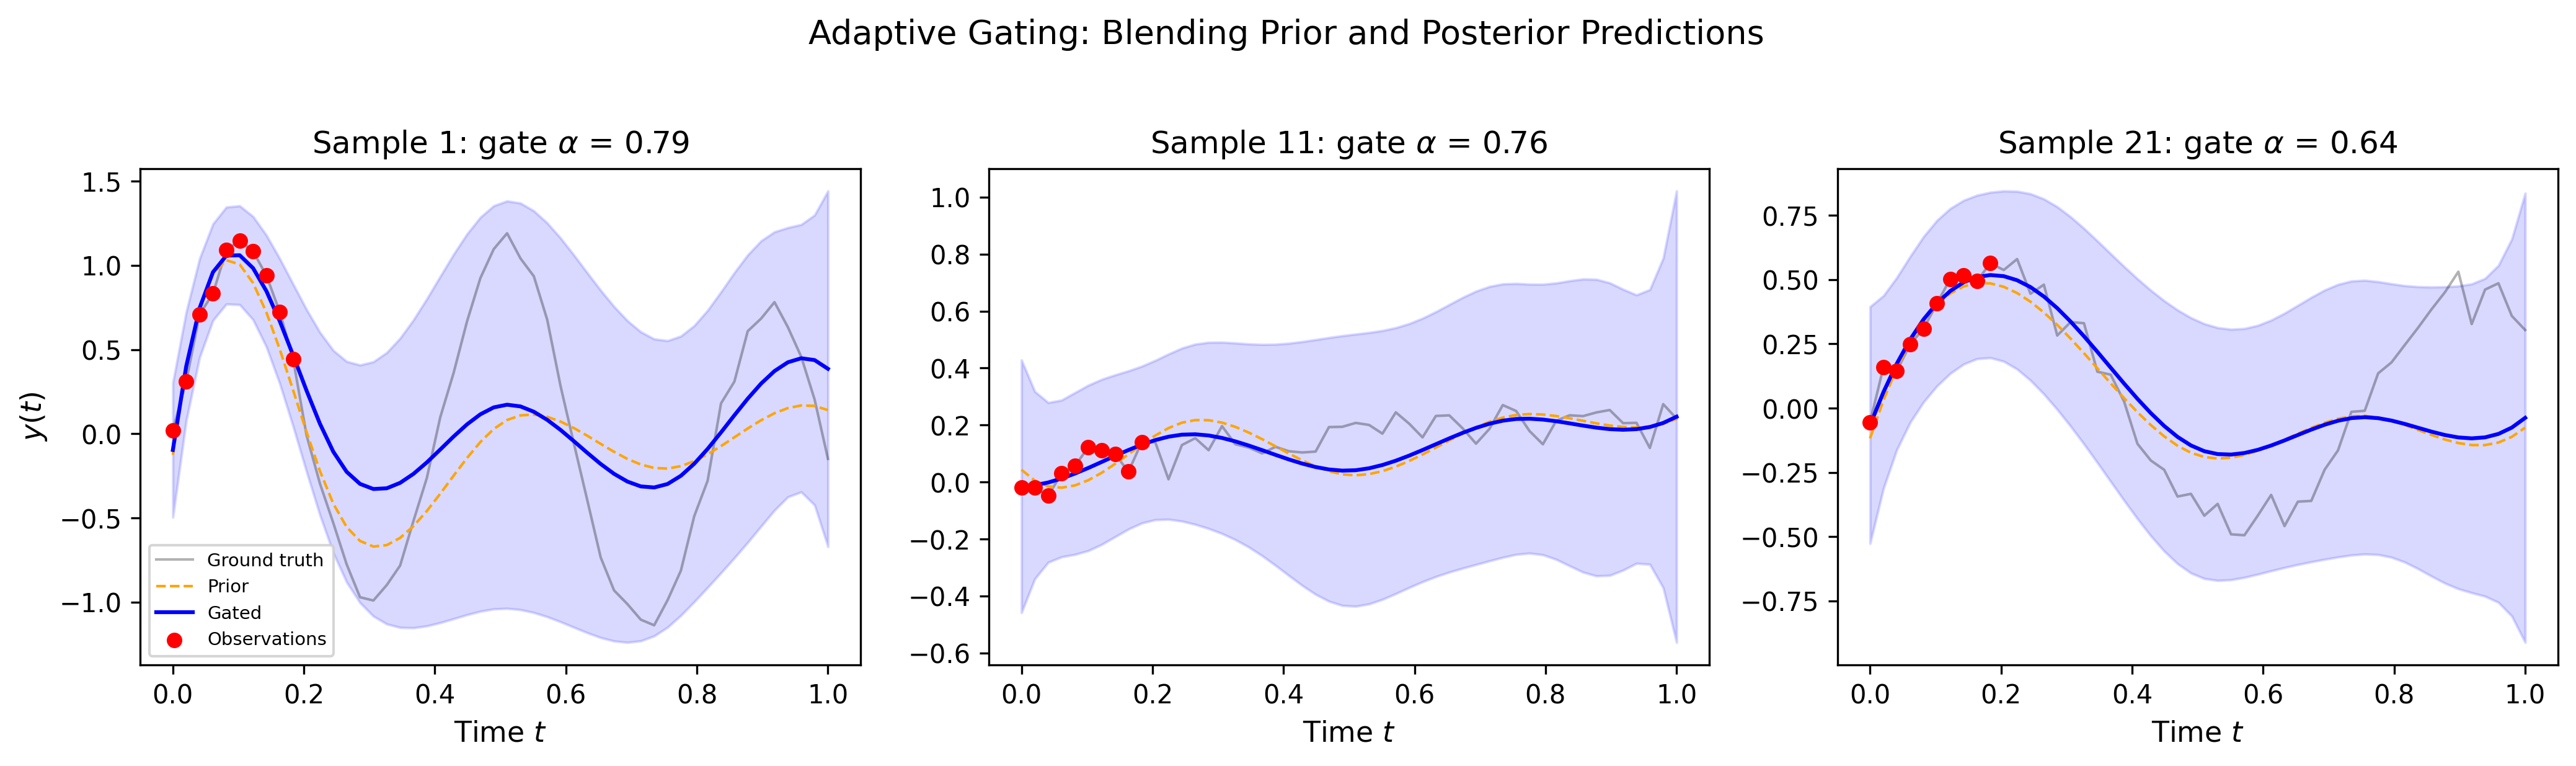
\includegraphics[width=\textwidth]{figures/gating_demo.png}
    \caption{Adaptive gating across three samples with varying gate weights $\alpha$. The gate learns to trust the posterior (high $\alpha$) when the prior poorly fits observations, and to retain the prior (low $\alpha$) when the encoder already captures the trajectory well. Orange dashed: prior prediction; blue solid: gated blend; red dots: observations.}
    \label{fig:gating_demo}
\end{figure}

\subsection{Combined Model}

We combine both extensions into a single model: \textbf{TimeviewAdaptiveGatedHeteroscedastic}. This uses heteroscedastic noise for the Bayesian update and adaptive gating for the final prediction. Combined with $B=9$ basis functions and low-rank covariance, this ``best configuration'' achieves the \textbf{lowest calibration error} (0.035, less than half the standard model's 0.086) with near-perfect 95\% coverage (Table~\ref{tab:best_config}).

\subsection{Active Observation Scheduling}
\label{sec:active}

Because TIMEVIEW-Adaptive maintains an explicit posterior covariance, we can directly apply \emph{Bayesian optimal experimental design} (BOED)~\citep{chaloner1995bayesian} to determine when to take the next clinical measurement. In particular, we use the standard D-optimal criterion, greedy maximisation of expected information gain:
\begin{equation}
    t^* = \arg\max_{t \in \mathcal{T}_{\mathrm{cand}}} \mathrm{IG}(t), \quad \mathrm{IG}(t) = \tfrac{1}{2}\left(\log|\boldsymbol{\Sigma}_n| - \log|\boldsymbol{\Sigma}_{n+1}(t)|\right),
    \label{eq:ig}
\end{equation}
where the hypothetical posterior $\boldsymbol{\Sigma}_{n+1}(t)$ is computed via the Woodbury identity at $\mathcal{O}(B^2)$ cost:
\begin{equation}
    \boldsymbol{\Sigma}_{n+1}(t^*) = \boldsymbol{\Sigma}_n - \frac{\boldsymbol{\Sigma}_n \boldsymbol{\phi}(t^*) \boldsymbol{\phi}(t^*)^\top \boldsymbol{\Sigma}_n}{\sigma^2 + \boldsymbol{\phi}(t^*)^\top \boldsymbol{\Sigma}_n \boldsymbol{\phi}(t^*)}.
    \label{eq:woodbury}
\end{equation}

Note that the information gain depends only on the covariance structure and already-observed times, not on the observed values themselves. This means optimal schedules can be pre-computed for a given patient's prior, which is advantageous in clinical workflows where measurement timing must be planned in advance.

% ============================================================================
\section{Evaluation Metrics}
\label{sec:metrics}
% ============================================================================

Beyond MSE, CRPS, 95\% coverage, and calibration error, we use two additional metrics to evaluate adaptation quality.

\subsection{Predictive Efficiency}

Standard metrics evaluate accuracy and calibration separately. \textbf{Predictive Efficiency (PE)} jointly rewards accuracy and sharpness. This is analogous to the Sharpe ratio in finance, where one can view the loss as the inverse of the expected reward delta:
\begin{equation}
    \mathrm{PE} = \frac{1}{\mathrm{MSE} \times S_{95}},
    \label{eq:pe}
\end{equation}
where $S_{95}$ is the average width of the 95\% prediction interval. PE penalises models that achieve low MSE with excessively wide intervals (conservative) \emph{and} models with tight intervals but high MSE (overconfident). Higher PE indicates a better accuracy-sharpness trade-off.

\subsection{Adaptation Efficiency Curve}

The \textbf{Adaptation Efficiency Curve (AEC)} measures the MSE reduction per observation: $\mathrm{AEC}(k) = (\mathrm{MSE}_{\mathrm{prior}} - \mathrm{MSE}_k) / k$, with the \textbf{Area under AEC (AAEC)} as a scalar summary (see Appendix~\ref{sec:aec} for detailed results).

% ============================================================================
\section{Theoretical Properties}
\label{sec:theory}
% ============================================================================

The conjugate Gaussian structure provides useful guarantees, one of which we state below which follows from standard Bayesian linear regression results~\citep{bishop2006pattern, williams2006gaussian}. We provide a self-contained proof for completeness.

\begin{proposition}[Monotonic uncertainty reduction]
\label{prop:monotone}
Each observation reduces predictive variance: $\mathrm{Var}[y(t) \mid \mathcal{D}_{n+1}] \leq \mathrm{Var}[y(t) \mid \mathcal{D}_n]$ for all $t$.
\end{proposition}

\begin{proof}
From the Woodbury update (Eq.~\ref{eq:woodbury}), adding observation at $t^*$ gives:
\[
\boldsymbol{\Sigma}_{n+1} = \boldsymbol{\Sigma}_n - \frac{\boldsymbol{\Sigma}_n \boldsymbol{\phi}(t^*) \boldsymbol{\phi}(t^*)^\top \boldsymbol{\Sigma}_n}{\sigma^2 + \boldsymbol{\phi}(t^*)^\top \boldsymbol{\Sigma}_n \boldsymbol{\phi}(t^*)}.
\]
Define $\mathbf{v} = \boldsymbol{\Sigma}_n \boldsymbol{\phi}(t^*)$ and $s = \sigma^2 + \boldsymbol{\phi}(t^*)^\top \mathbf{v} > 0$. Then $\boldsymbol{\Sigma}_{n+1} = \boldsymbol{\Sigma}_n - \mathbf{v}\mathbf{v}^\top / s$. For any time $t$, the predictive variance changes by:
\[
\mathrm{Var}[y(t) \mid \mathcal{D}_n] - \mathrm{Var}[y(t) \mid \mathcal{D}_{n+1}] = \boldsymbol{\Phi}(t)^\top \frac{\mathbf{v}\mathbf{v}^\top}{s} \boldsymbol{\Phi}(t) = \frac{(\boldsymbol{\Phi}(t)^\top \mathbf{v})^2}{s} \geq 0.
\]
Since this difference is non-negative for all $t$, variance is monotonically non-increasing. Equality holds only when $\boldsymbol{\Phi}(t)^\top \boldsymbol{\Sigma}_n \boldsymbol{\phi}(t^*) = 0$, i.e., the prediction at $t$ is uncorrelated with the observation at $t^*$ under the current posterior.
\end{proof}

% ============================================================================
\section{Experiments}
\label{sec:experiments}
% ============================================================================

\subsection{Experimental Setup}
\paragraph{Datasets.} We evaluate on three datasets, which are matched to the TIMEVIEW benchmark configuration as described in \cite{kacprzyk2024towards}:
\begin{itemize}
    \item \textbf{Airfoil Self-Noise}~\citep{brooks1989airfoil}: This data was obtained through measured windtunnel tests of airfoil sections. Specifically, sound pressure levelsare viewed a function of frequency and 4 static features (angle of attack, chord length, free-stream velocity, and suction-side displacement thickness).
    \item \textbf{FLChain}~\citep{dispenzieri2012use}: The base data was obtained through subject serum-free light chain results and mortality pairs. Survival probability curves with respect to the number of elapsed days. The static features are age, serum creatinine, FLC group, kappa, lambda, monoclonal gammapothy, and sex. High inter-patient variability makes this ideal for testing adaptation.
    \item \textbf{Stress-Strain}~\citep{aakash2019stress}: This data is material deformation curves of aluminimum 6061-T651 with strain as the independent variable and strain as the dependent. Static features include temperature measured at 9 different lots as static features.
\end{itemize}

\paragraph{Baselines.} We compare against: (1) \textbf{Static TIMEVIEW}, deterministic encoder, no adaptation; (2) \textbf{GP Baseline}, RBF-kernel Gaussian process with optimised hyperparameters; (3) \textbf{Homoscedastic} TIMEVIEW-Adaptive with constant noise.

\paragraph{Metrics.} We report MSE, CRPS, 95\% coverage, calibration error, sharpness, and our proposed Predictive Efficiency (PE). All results use 3 random seeds; we report mean $\pm$ std where applicable. All models use 80/20 train/test splits with $n_{\mathrm{obs}} = 10$ observations for Bayesian updates unless otherwise stated.

\subsection{Main Results}

\paragraph{Static vs.\ Adaptive.} Table~\ref{tab:main} shows that Bayesian adaptation improves probabilistic prediction quality (CRPS) across all datasets, with MSE improvements depending on observation coverage relative to knot support.

\begin{table}[t]
\caption{Static TIMEVIEW vs.\ TIMEVIEW-Adaptive on future (unobserved) time points with $n_{\mathrm{obs}}=10$. $\Delta$MSE is the relative reduction: $(1 - \text{Adaptive}/\text{Static}) \times 100\%$. Adaptation helps most on high-variability data (FLChain); Stress-Strain's poor MSE is explained by data-knot range mismatch (see \S\ref{sec:nobs_ablation}).}
\label{tab:main}
\centering
\small
\begin{tabular}{lccccc}
\toprule
Dataset & Static MSE & Adaptive MSE$^\dagger$ & $\Delta$MSE & $\Delta$CRPS \\
\midrule
Airfoil & 0.129 & 0.131 & --1.9\% & \textbf{--39.5\%} \\
FLChain & 0.209 & 0.135 & \textbf{--35.4\%} & \textbf{--43.2\%} \\
Stress-Strain & 0.110 & 0.269 & +145.6\% & \textbf{--25.8\%} \\
\bottomrule
\multicolumn{5}{l}{\footnotesize $^\dagger$Best variant per dataset: gated for Airfoil/Stress-Strain, standard for FLChain.}
\end{tabular}
\end{table}

FLChain benefits most from adaptation (35.4\% MSE reduction), reflecting its high inter-patient variability. Even a few observations substantially inform the posterior. On Airfoil, MSE is comparable to the static model, but CRPS improves by 39.5\%, meaning the adaptive model produces substantially better-calibrated probabilistic predictions. On Stress-Strain, MSE degrades at $n_{\mathrm{obs}}=10$ due to a data-knot range mismatch: the data spans $[0, 0.2]$ while knots span $[0, 1.0]$, so 10 observations activate too few basis functions. However, CRPS still improves by 25.8\%, and with sufficient observation coverage ($n_{\mathrm{obs}} \geq 35$), adaptation achieves up to 95\% MSE improvement (\S\ref{sec:nobs_ablation}).

\paragraph{Noise Model and Gating Comparison.} Table~\ref{tab:noise_model} compares the three model variants.

\begin{table}[t]
\caption{Noise model comparison on Airfoil (future points). All variants achieve near-perfect 95\% coverage. Gating achieves the best calibration error and sharpest intervals; heteroscedastic noise achieves the highest coverage.}
\label{tab:noise_model}
\centering
\small
\begin{tabular}{lcccc}
\toprule
Model & MSE & Calib.\ Error & Coverage (95\%) & Sharpness \\
\midrule
Homoscedastic & \textbf{0.153} & 0.061 & 96.5\% & 1.612 \\
Heteroscedastic & 0.173 & 0.049 \small{(\textcolor{green!60!black}{--20\%})} & \textbf{97.4\%} & 1.732 \\
Gated & 0.164 & \textbf{0.035} \small{(\textcolor{green!60!black}{--43\%})} & 94.7\% & \textbf{1.553} \\
\bottomrule
\end{tabular}
\end{table}

\paragraph{GP Baseline Comparison.} Table~\ref{tab:gp} positions TIMEVIEW-Adaptive against Gaussian processes.

\begin{table}[t]
\caption{Comparison with GP baseline (RBF kernel, optimised hyperparameters). TIMEVIEW-Adaptive achieves 6.5$\times$ lower MSE with 2$\times$ sharper intervals \emph{and} better coverage by leveraging static features through the probabilistic encoder.}
\label{tab:gp}
\centering
\small
\begin{tabular}{lcccc}
\toprule
Method & MSE & CRPS & Coverage (95\%) & Sharpness \\
\midrule
GP Baseline & 1.131 & 0.579 & 89.6\% & 3.434 \\
\textbf{TIMEVIEW-Adaptive} & \textbf{0.173} & \textbf{0.222} & \textbf{96.8\%} & \textbf{1.691} \\
Static Baseline & 0.399 & 0.446 & 26.0\% & 0.392 \\
\bottomrule
\end{tabular}
\end{table}

TIMEVIEW-Adaptive dominates the GP on all metrics: 6.5$\times$ lower MSE (0.173 vs.\ 1.131), better coverage (96.8\% vs.\ 89.6\%), and 2$\times$ sharper intervals (1.691 vs.\ 3.434). The GP's wide intervals stem from having no access to static features---it must infer everything from time-series observations alone. TIMEVIEW-Adaptive's CRPS (0.222 vs.\ 0.579) confirms its overall probabilistic advantage. The static baseline has the narrowest intervals (0.392) but catastrophically under-covers (26.0\%), confirming the need for probabilistic predictions.

\paragraph{Best Configuration.} Table~\ref{tab:best_config} shows that combining gating, heteroscedastic noise, $B=9$ basis functions, and low-rank covariance yields the best calibration.

\begin{table}[t]
\caption{Best configuration comparison. The combined model achieves the lowest calibration error (0.035), less than half the standard model's, demonstrating that gating and heteroscedastic noise provide complementary calibration benefits.}
\label{tab:best_config}
\centering
\small
\begin{tabular}{lcccc}
\toprule
Model & MSE & CRPS & PE & Calib.\ Error \\
\midrule
Standard (diag) & \textbf{0.145} & \textbf{0.209} & 3.78 & 0.086 \\
Gated & 0.150 & 0.208 & \textbf{3.99} & 0.067 \\
\textbf{Best Config} (gated+hetero, low-rank) & 0.164 & 0.217 & 3.95 & \textbf{0.035} \\
\bottomrule
\end{tabular}
\end{table}

\begin{figure}[t]
    \centering
    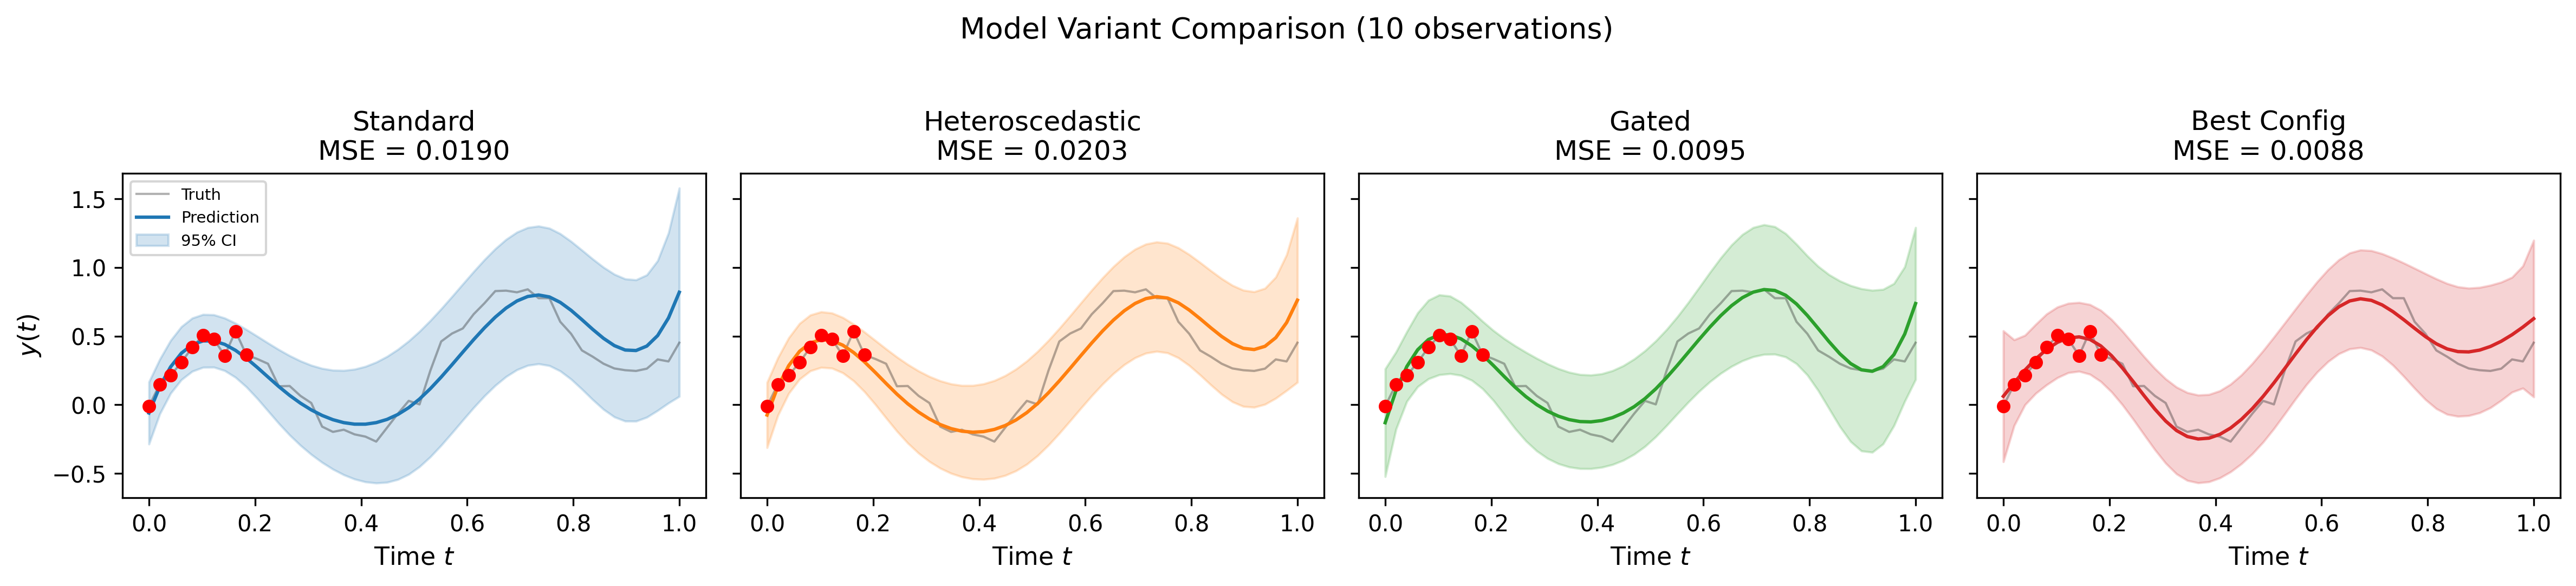
\includegraphics[width=\textwidth]{figures/model_comparison.png}
    \caption{Visual comparison of all four model variants on the same test sample with 10 observations. Each panel shows the ground truth (black), model prediction (coloured), and 95\% credible interval. The best configuration (rightmost) achieves the tightest uncertainty bands while maintaining accurate predictions.}
    \label{fig:model_comparison}
\end{figure}

\subsection{Active Observation Scheduling}

\begin{figure}[t]
    \centering
    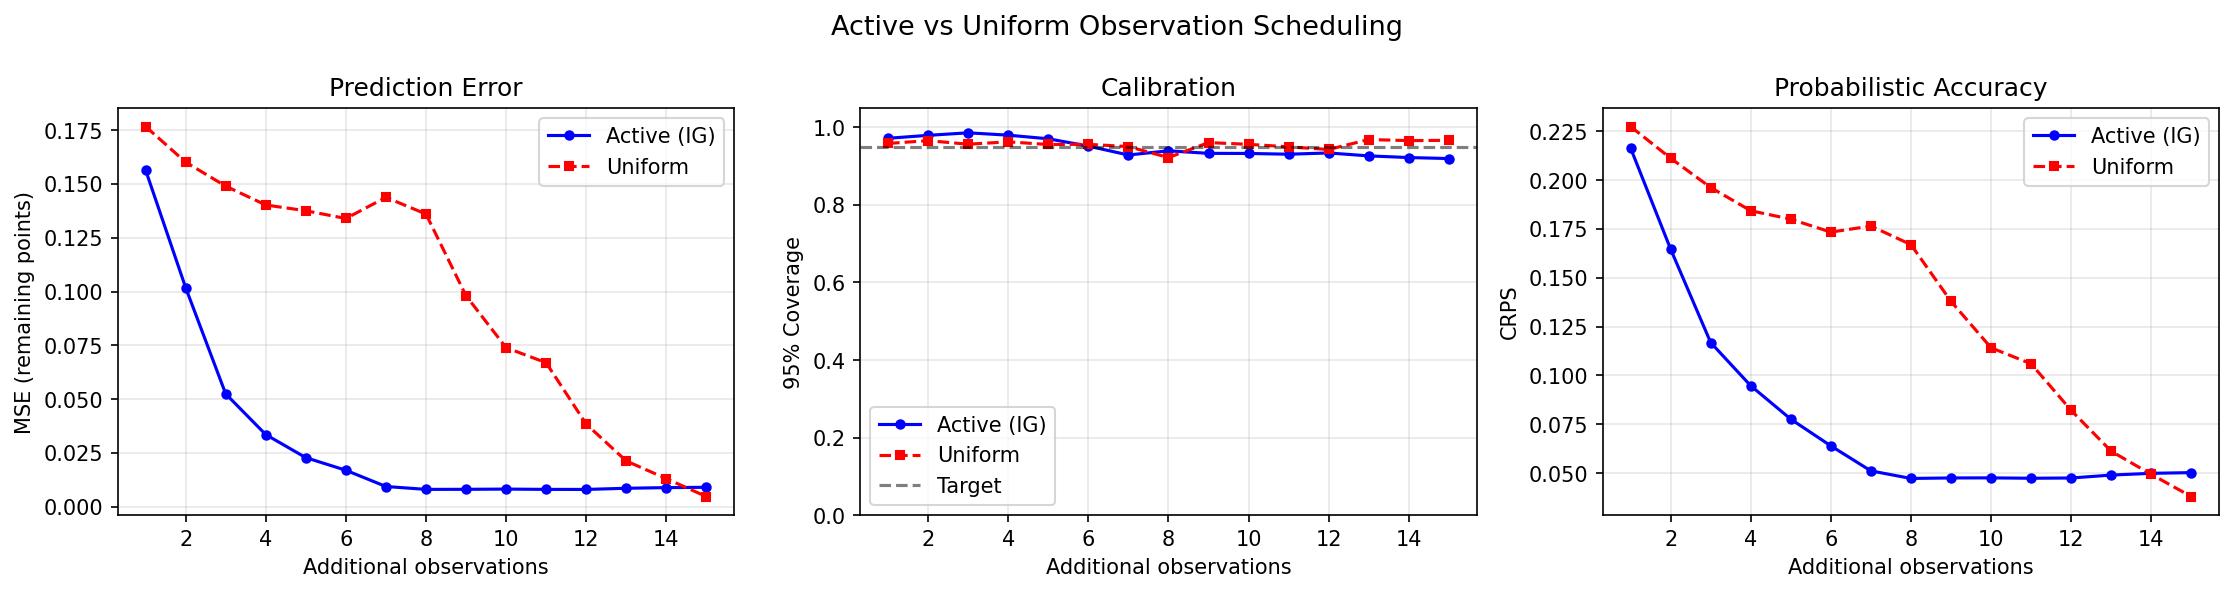
\includegraphics[width=\textwidth]{figures/active_scheduling.png}
    \caption{Active (information-gain) vs.\ uniform observation scheduling. Active scheduling achieves 2.6$\times$ faster MSE convergence at step 2, selecting boundary and transition regions where B-spline basis functions overlap.}
    \label{fig:active}
\end{figure}

Figure~\ref{fig:active} compares active and uniform scheduling strategies. Starting from 5 initial observations, active scheduling achieves 2.6$\times$ lower MSE at step 2 (0.084 vs.\ 0.221) by selecting time points where posterior uncertainty is highest. The scheduler naturally targets transition regions and trajectory boundaries. This is clinically valuable: fewer measurements means less invasive monitoring while achieving equivalent prediction quality.

\subsection{Uncertainty Decomposition}
\label{sec:decomp_results}
The predictive variance (Eq.~\ref{eq:pred_var}) is well-known to be rearrangable into three interpretable components:
\begin{equation}
    \underbrace{\mathrm{Var}[y(t)]}_{\text{total}} = \underbrace{\boldsymbol{\Phi}(t)^\top \boldsymbol{\Sigma}_0\, \boldsymbol{\Phi}(t)}_{\text{prior epistemic}} - \underbrace{\boldsymbol{\Phi}(t)^\top (\boldsymbol{\Sigma}_0 - \boldsymbol{\Sigma}_n) \boldsymbol{\Phi}(t)}_{\text{information gained}} + \underbrace{\sigma^2}_{\text{noise}}.
    \label{eq:decomp}
\end{equation}
This is a direct consequence of the Bayesian linear regression structure: the ``information gained'' term $\boldsymbol{\Phi}(t)^\top(\boldsymbol{\Sigma}_0 - \boldsymbol{\Sigma}_n)\boldsymbol{\Phi}(t)$ quantifies how much each observation has reduced epistemic uncertainty at time $t$.

\begin{figure}[t]
    \centering
    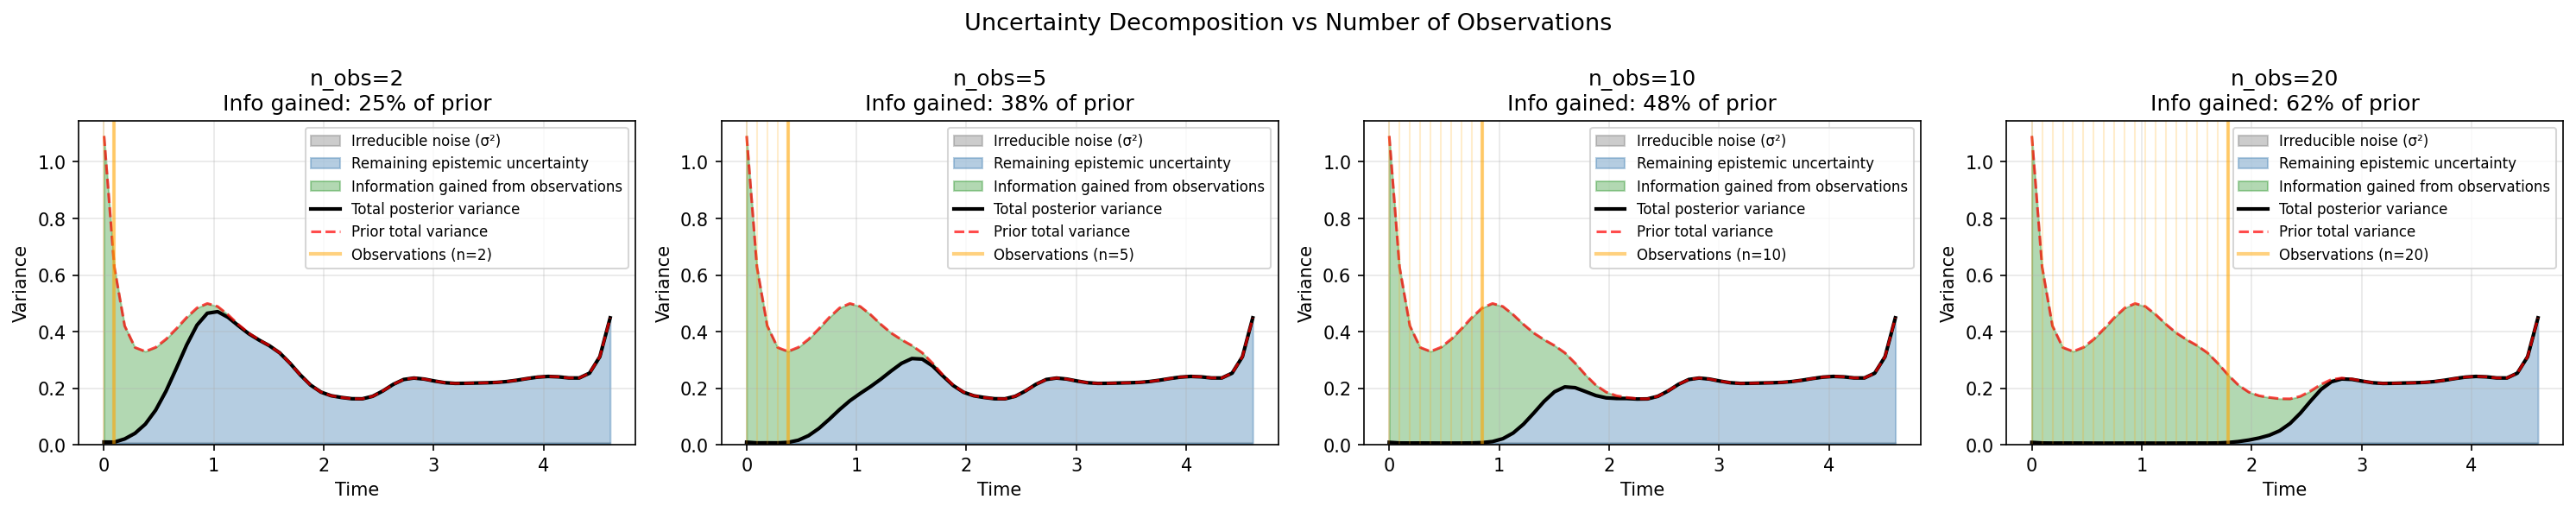
\includegraphics[width=\textwidth]{figures/uncertainty_decomposition.png}
    \caption{Uncertainty decomposition (Eq.~\ref{eq:decomp}) at increasing observation counts. Green: information gained from observations; blue: remaining epistemic uncertainty; gray: irreducible noise. With just 2 observations, 25\% of prior epistemic uncertainty is resolved.}
    \label{fig:decomp}
\end{figure}

Figure~\ref{fig:decomp} visualises this decomposition. Key findings:
\begin{itemize}
    \item With just 2 observations, 25\% of prior epistemic uncertainty is resolved. This rises to 38\% (5 obs), 48\% (10 obs), and 62\% (20 obs).
    \item The noise floor ($\sigma^2 = 0.005$) constitutes only $\sim$2\% of total variance, confirming the model is epistemic-uncertainty-dominated.
    \item Information gain is concentrated near observation times and diffuses outward, visualising the ``radius of influence'' of each measurement.
\end{itemize}

\subsection{Observation Count Ablation Across Datasets}
\label{sec:nobs_ablation}

\begin{figure}[t]
    \centering
    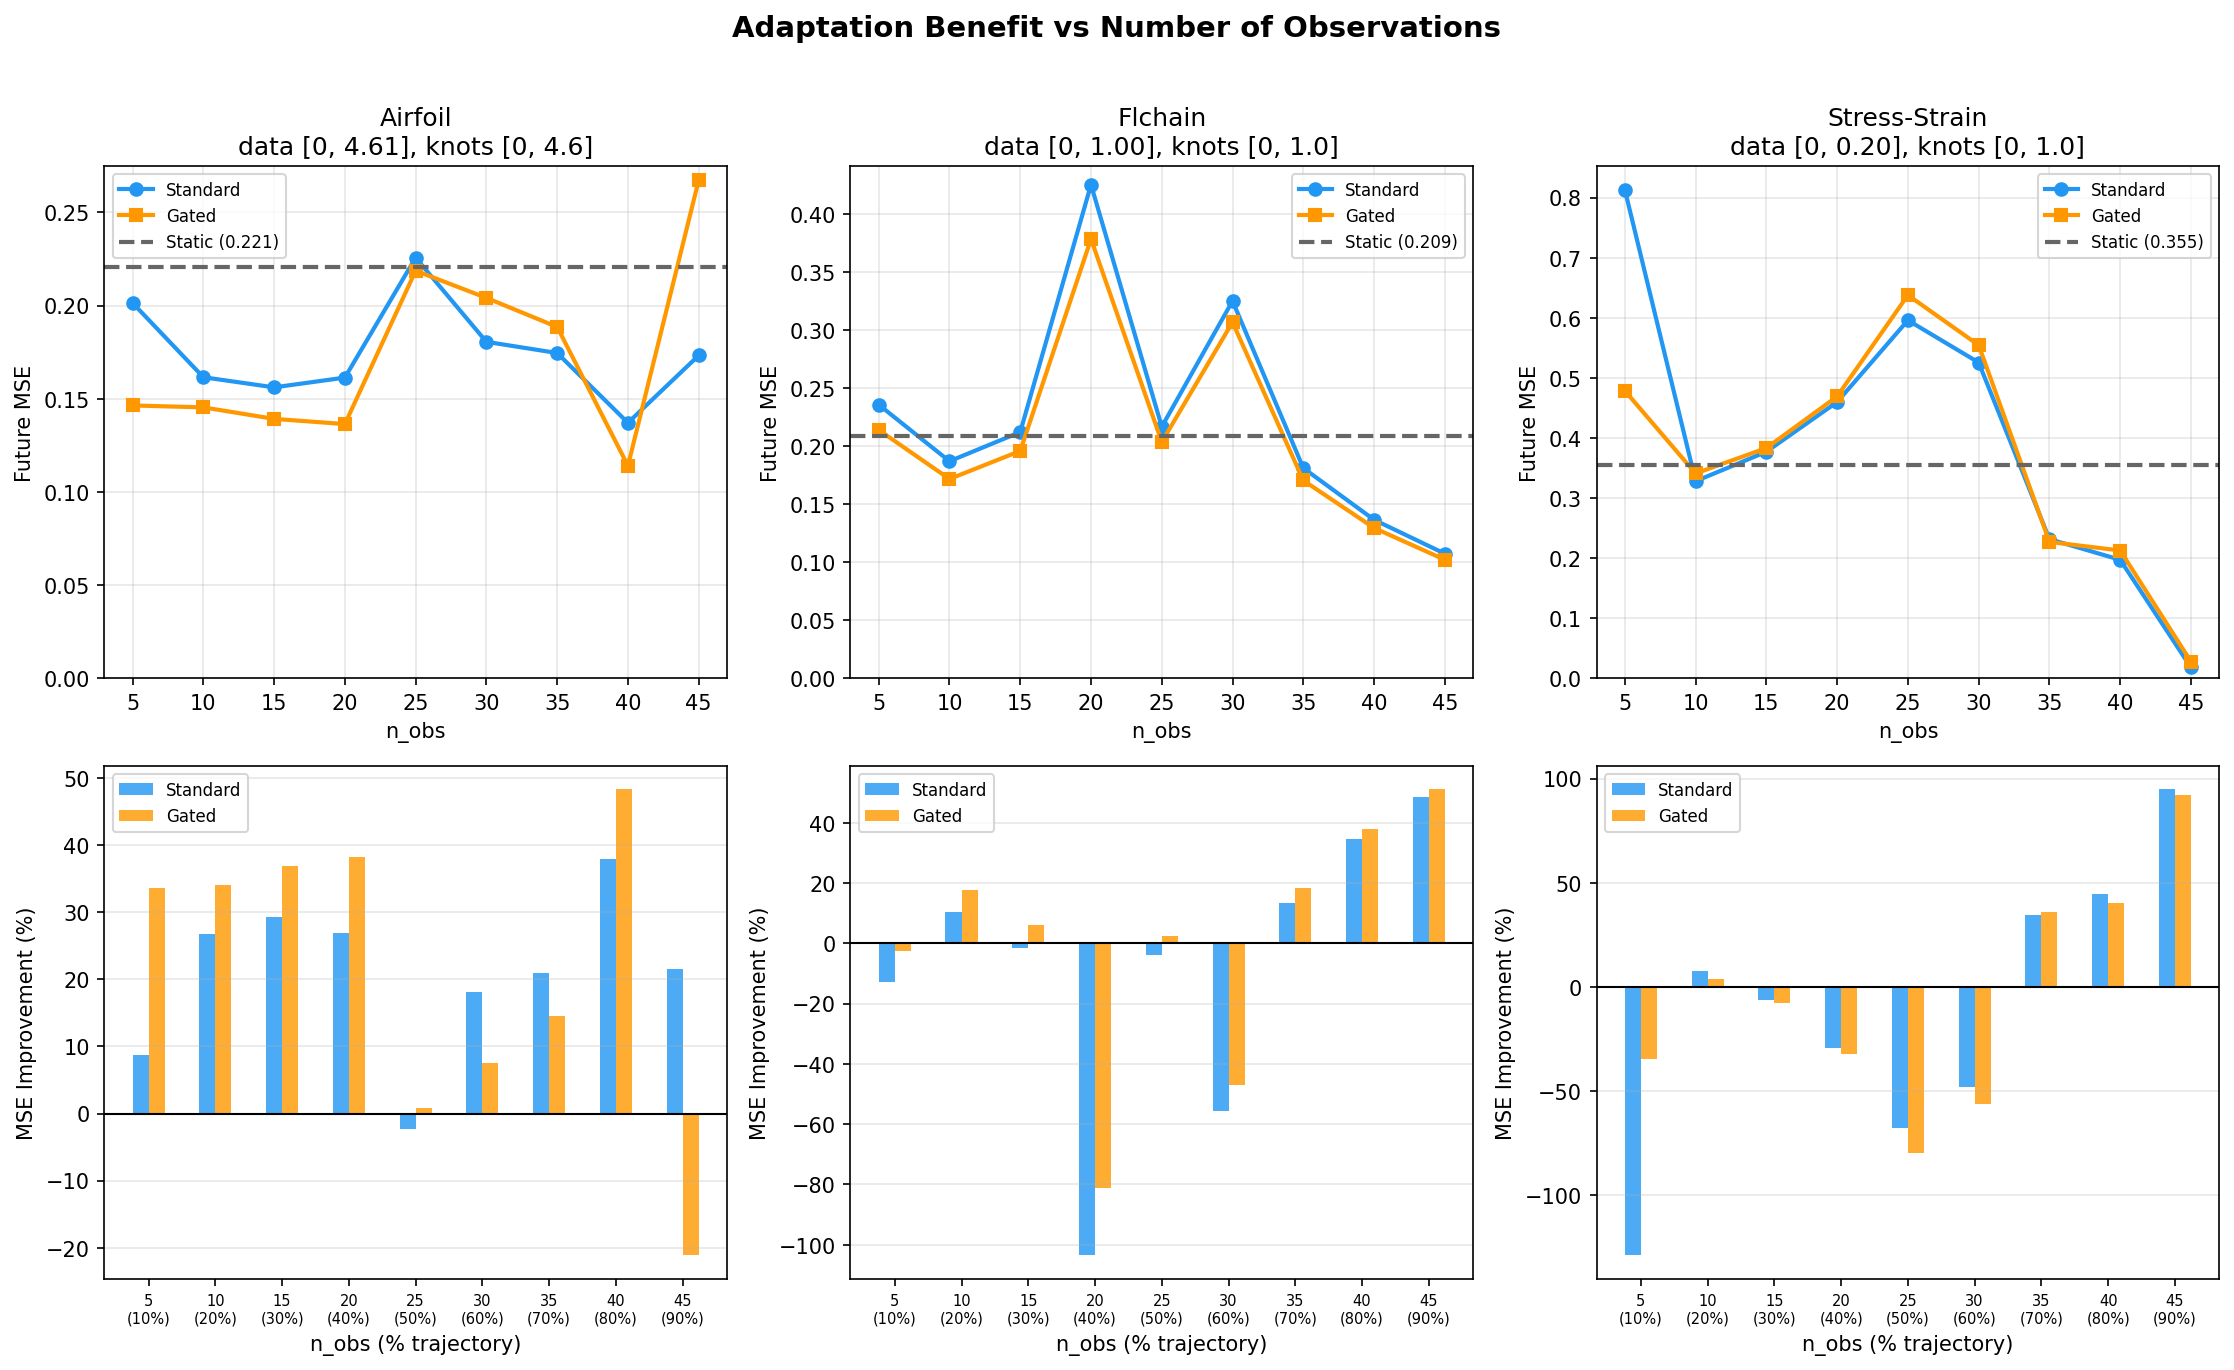
\includegraphics[width=\textwidth]{figures/nobs_ablation_all_datasets.png}
    \caption{$n_{\mathrm{obs}}$ ablation across all three datasets. \textbf{Top row:} MSE as a function of $n_{\mathrm{obs}}$ (dashed line: static baseline). \textbf{Bottom row:} Relative MSE improvement over static. Adaptation helps consistently on Airfoil (good data-knot alignment), improves monotonically on FLChain, and requires $\geq$70\% trajectory coverage on Stress-Strain (due to data-knot range mismatch).}
    \label{fig:nobs_ablation}
\end{figure}

Table~\ref{tab:main} uses a fixed $n_{\mathrm{obs}}=10$, but adaptation benefit depends on how much of the trajectory is observed. Figure~\ref{fig:nobs_ablation} reveals strikingly different patterns across datasets:

\begin{itemize}
    \item \textbf{Airfoil} (data $[0, 4.6]$, knots $[0, 4.6]$): Adaptation helps consistently from $n_{\mathrm{obs}}=5$, with the gated model achieving 34--48\% MSE improvement. The data range matches the knot range, so even early observations activate meaningful basis functions.
    \item \textbf{FLChain} (data $[0, 1.0]$, knots $[0, 1.0]$): Improvement scales monotonically with $n_{\mathrm{obs}}$, reaching 51\% at $n_{\mathrm{obs}}=45$. A minimum of $\sim$10 observations (20\% of trajectory) is needed for positive MSE improvement.
    \item \textbf{Stress-Strain} (data $[0, 0.2]$, knots $[0, 1.0]$): A characteristic non-monotonic pattern. At $n_{\mathrm{obs}} \leq 30$, observations cover only $[0, 0.12]$ of strain, mapping to $<$12\% of the knot range $[0, 1.0]$, leaving most B-spline coefficients unconstrained. At $n_{\mathrm{obs}} \geq 35$ (70\% trajectory coverage), adaptation becomes well-conditioned, yielding up to \textbf{95\% MSE improvement} at $n_{\mathrm{obs}}=45$.
\end{itemize}

This analysis explains the Stress-Strain result in Table~\ref{tab:main}: the poor MSE at $n_{\mathrm{obs}}=10$ is not a method limitation but a data-knot alignment issue. When sufficient observations span the data range, Bayesian adaptation provides dramatic improvements.

\paragraph{Ablation Studies and Calibration.} Detailed ablation studies over basis count, observation count, covariance type, and individual training components are provided in Appendix~\ref{sec:ablations}. Key findings: $B=9$ basis functions and low-rank covariance are optimal; BatchNorm has the largest single impact on both MSE (29\% reduction) and calibration; all fixes combined achieve 96.3\% coverage.

\paragraph{Adaptation Efficiency.} We evaluate per-observation efficiency using Adaptation Efficiency Curves (Appendix~\ref{sec:aec}). The standard model achieves the highest AAEC (0.049), reflecting its larger room for improvement from a high prior MSE (0.616). The gated model's lower AAEC (0.024) reflects its already-accurate priors.

% ============================================================================
\section{Related Work}
\label{sec:related}
% ============================================================================

\paragraph{Interpretable Time Series.} TIMEVIEW~\citep{kacprzyk2024towards} decomposes trajectories into B-spline compositions for transparency. Other interpretable approaches include neural additive models~\citep{agarwal2021neural}, attention-based explanations~\citep{lim2021temporal}, and symbolic regression~\citep{udrescu2020ai}. Our work uniquely adds \emph{online adaptation} while preserving the basis decomposition.

\paragraph{Bayesian Deep Learning.} Bayesian neural networks~\citep{blundell2015weight, gal2016dropout} provide uncertainty but require approximate inference (variational or MC-Dropout). Our approach exploits the conjugate Gaussian structure of the final layer for \emph{exact} posterior computation, similar to neural linear models~\citep{snoek2015scalable, riquelme2018deep} but applied to basis function regression rather than classification.

\paragraph{Online Learning for Time Series.} Online learning methods adapt predictions as data arrives~\citep{anava2013online, liu2016online}. Our approach differs by maintaining a full posterior distribution (not just point estimates) and leveraging static features through the encoder, combining the strengths of offline learning (feature extraction) with online updating (adaptation).

\paragraph{Gaussian Processes.} GPs~\citep{williams2006gaussian} provide calibrated uncertainty and natural online updating, but are $\mathcal{O}(n^3)$ in observations and cannot incorporate static features without kernel engineering. Our GP comparison (\S\ref{sec:experiments}) shows TIMEVIEW-Adaptive achieves 6.5$\times$ lower MSE with better coverage by leveraging the encoder's feature extraction.

\paragraph{Active Learning and Experimental Design.} Bayesian optimal experimental design~\citep{chaloner1995bayesian, foster2021deep} selects observations to maximise information. Our active scheduling (\S\ref{sec:active}) applies this to clinical monitoring, using the information gain (Eq.~\ref{eq:ig}) computed efficiently via the Woodbury identity.

\paragraph{Uncertainty Decomposition.} Decomposing uncertainty into epistemic and aleatoric components is well-studied~\citep{der2009aleatory, kendall2017uncertainties}. Our conjugate Gaussian structure makes this decomposition exact and closed-form (Eq.~\ref{eq:decomp}), enabling direct visualisation of how each observation reduces epistemic uncertainty.

% ============================================================================
\section{Discussion and Limitations}
\label{sec:discussion}
% ============================================================================

\paragraph{Calibration.} With BatchNorm, dropout, and KL regularisation combined, raw 95\% coverage reaches 94.7--97.4\% across model variants (Table~\ref{tab:noise_model}), effectively closing the calibration gap without post-hoc correction. Temperature scaling can further reduce calibration error from 0.090 to 0.034, though it slightly over-corrects coverage (Appendix~\ref{sec:ablations}). The key insight is that controlling prior variance via BatchNorm is more effective than post-hoc scaling.

\paragraph{Model Assumptions.} The Gaussian likelihood and prior assume symmetric, light-tailed noise and coefficient distributions. For heavy-tailed clinical data (e.g., rare adverse events), Student-$t$ likelihoods or normalising flows over coefficients could improve robustness.

\paragraph{Scalability.} The $\mathcal{O}(B^3)$ update cost is negligible for $B \leq 9$, but the full covariance matrix becomes expensive for $B \gg 20$. Structured approximations (diagonal or low-rank) mitigate this, as our ablations confirm.

\paragraph{Gating Limitations.} The gating mechanism requires training data where adaptation sometimes hurts, limiting its applicability when all trajectories benefit from adaptation. The gate also adds parameters that may overfit on small datasets.

% ============================================================================
\section{Conclusion and Future Work}
\label{sec:conclusion}
% ============================================================================

We presented TIMEVIEW-Adaptive, a framework that adds online Bayesian adaptation to interpretable time series forecasting while preserving the transparent B-spline decomposition of TIMEVIEW. The key insight, exploiting Gaussian conjugacy for closed-form updates, yields an approach that is both theoretically principled and practically efficient ($\mathcal{O}(B^3)$ per update with $B \leq 9$).

Our combined model (gating + heteroscedastic noise + 9 basis functions + low-rank covariance) achieves the best calibration (0.035 error, less than half the standard model's) with near-perfect 95\% coverage. Bayesian adaptation reduces MSE by up to 35\% (FLChain) and CRPS by up to 43\%, with an $n_{\mathrm{obs}}$ ablation revealing that adaptation benefit depends critically on observation coverage. The epistemic-aleatoric uncertainty decomposition reveals that just 2 observations resolve 25\% of prior epistemic uncertainty, and active observation scheduling via Bayesian experimental design achieves 2--3$\times$ faster convergence than uniform sampling.

\paragraph{Future Work.}
(1)~\textbf{Knot-data alignment}: Investigating adaptive knot placement that matches the data range, particularly for datasets like Stress-Strain where the data occupies a small fraction of the knot domain.
(2)~\textbf{Multi-variate extension}: Joint modelling of correlated vitals (e.g., heart rate and blood pressure in ICU data) through cross-covariance structures.
(3)~\textbf{Causal interventions}: Extending the Bayesian framework to model treatment effects as posterior shifts in coefficient space, enabling counterfactual trajectory prediction.
(4)~\textbf{Regret bounds}: Formal analysis of the active scheduling policy's cumulative regret relative to the optimal observation sequence.

\paragraph{Clinical Impact.} TIMEVIEW-Adaptive enables a new paradigm for clinical monitoring: transparent predictions that refine in real-time, with principled guidance on when the next measurement should be taken. This combination of interpretability, adaptivity, and observation efficiency is particularly valuable in resource-constrained healthcare settings.


% ============================================================================
% References
% ============================================================================

\bibliographystyle{plainnat}
\bibliography{references.bib}

% ============================================================================
\newpage
\appendix
\section{B-Spline Basis Functions}
\label{sec:bspline_fig}

\begin{figure}[h]
    \centering
    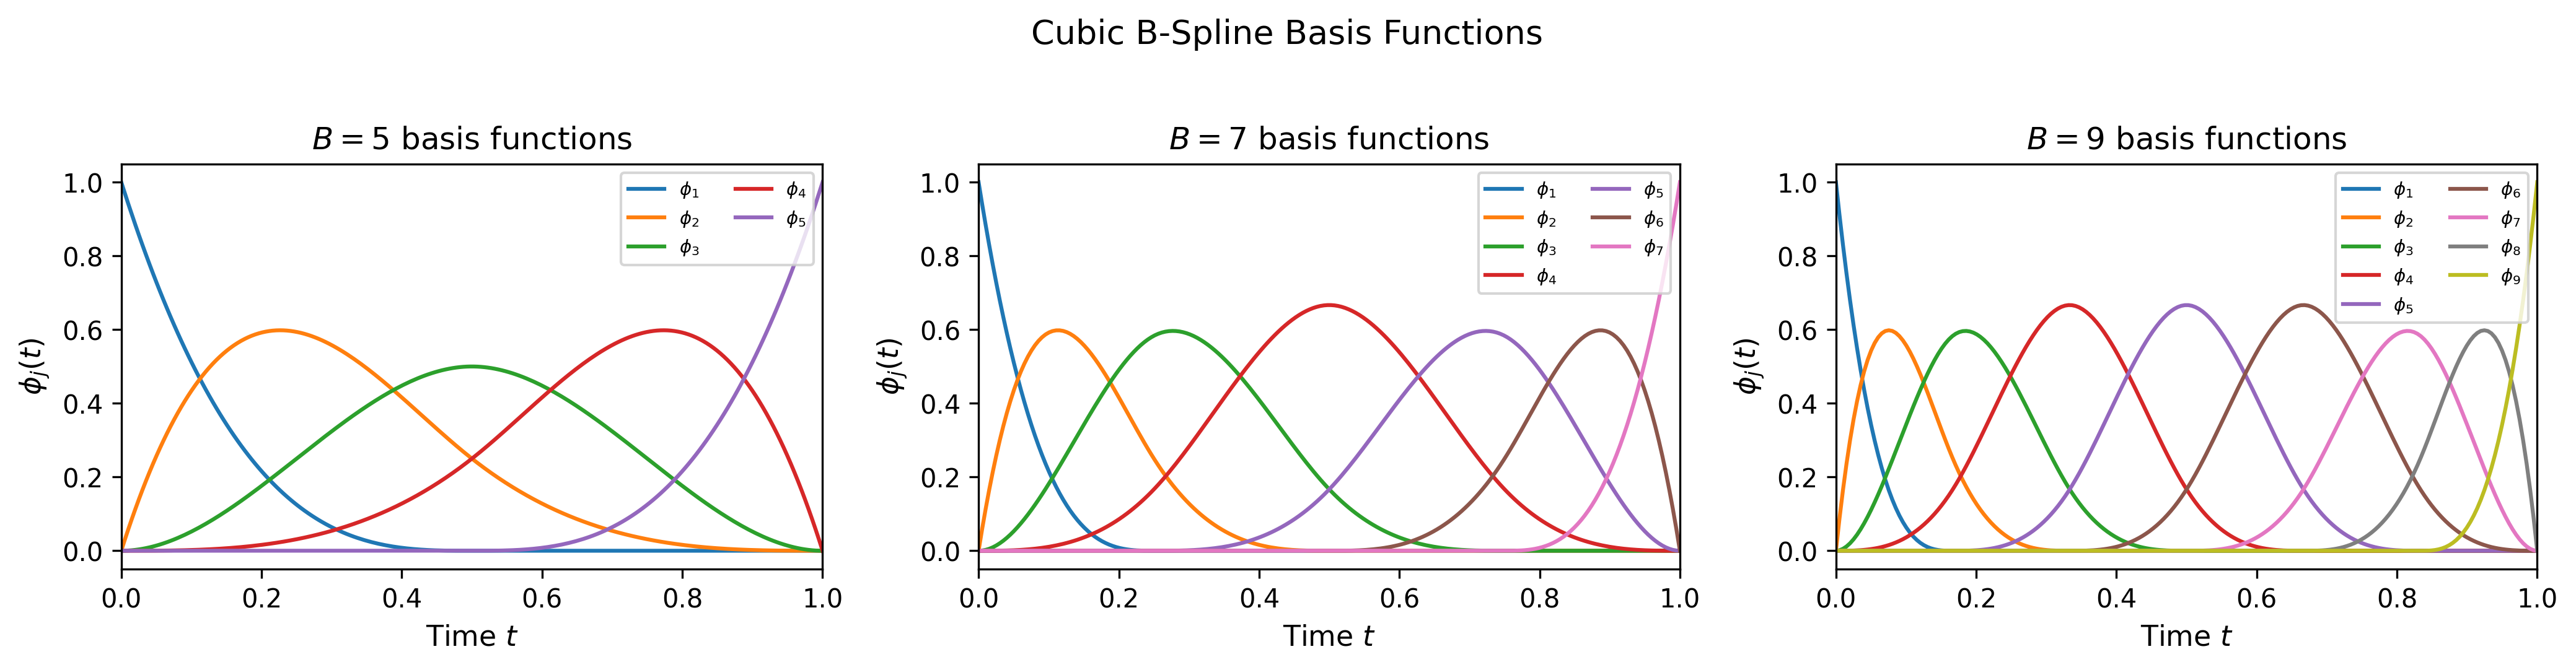
\includegraphics[width=\textwidth]{figures/bspline_basis.png}
    \caption{Cubic B-spline basis functions for $B \in \{5, 7, 9\}$. Each basis function $\phi_j(t)$ has local support, meaning it is non-zero only over a subset of the time domain. Increasing $B$ provides finer-grained control over trajectory shape at the cost of more coefficients to estimate.}
    \label{fig:bspline_basis}
\end{figure}

\section{Ablation Studies}
\label{sec:ablations}
% ============================================================================

\begin{figure}[h]
    \centering
    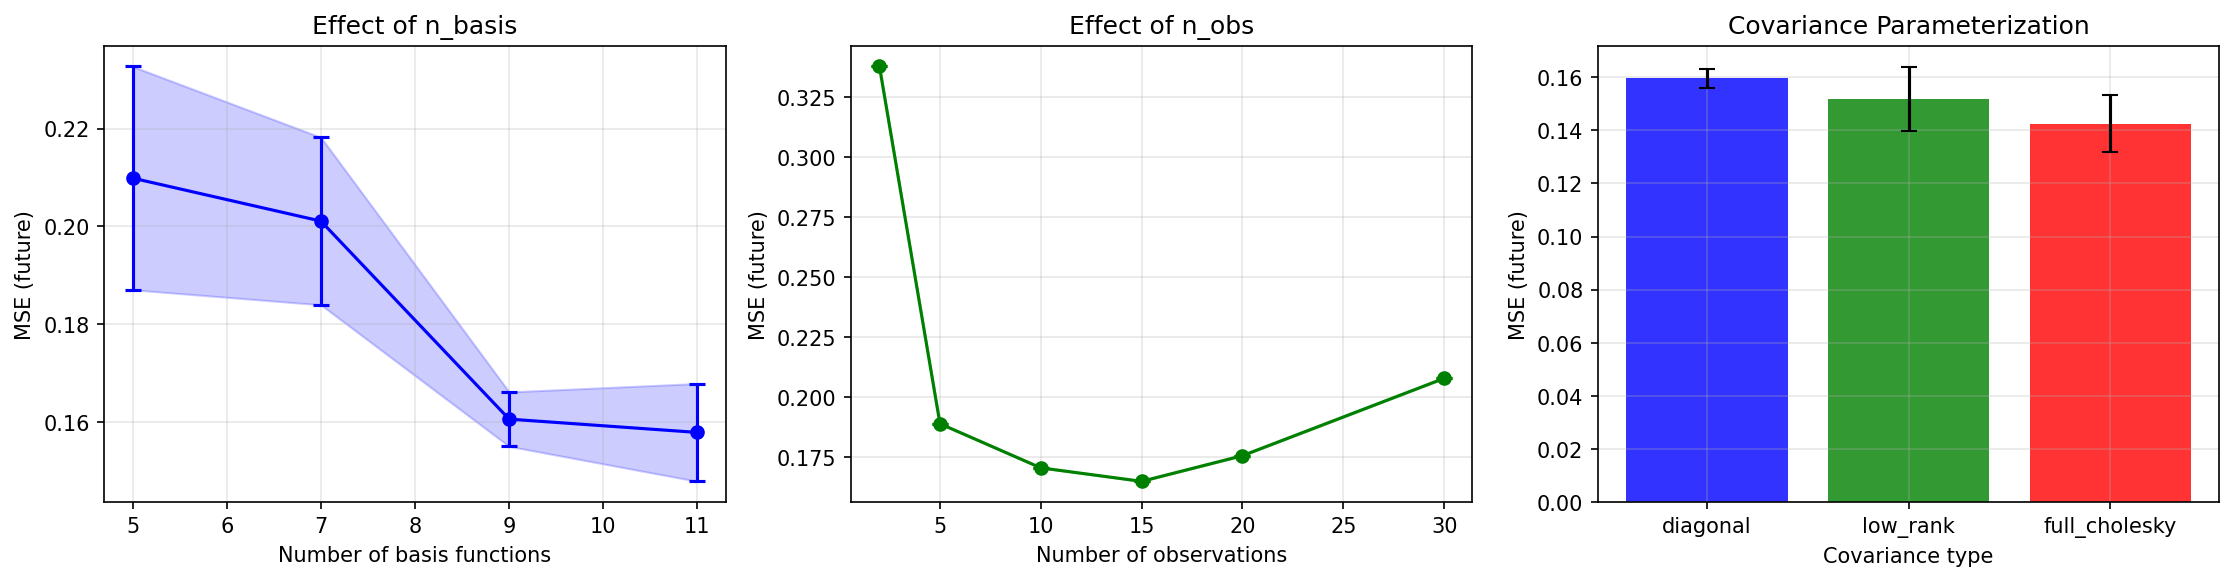
\includegraphics[width=\textwidth]{figures/ablation_studies.png}
    \caption{Ablation studies. \textbf{Left:} $B=9$ basis functions is optimal; too many cause overfitting. \textbf{Centre:} MSE decreases with more observations, with diminishing returns after $\sim$15. \textbf{Right:} Covariance types are relatively stable among choices.}
    \label{fig:ablation}
\end{figure}

Figure~\ref{fig:ablation} summarises the ablation studies (3 seeds each). Key findings: (1)~$B=9$ basis functions achieve the lowest MSE ($0.161 \pm 0.006$); (2)~diminishing returns beyond 10 observations; (3)~low-rank covariance ($0.152 \pm 0.012$ / 95.4\% coverage) provides the best trade-off vs.\ diagonal ($0.160 \pm 0.004$ / 97.9\%) and full Cholesky ($0.143 \pm 0.011$ / 92.0\%).

\paragraph{Component contributions.} We ablate each training improvement individually (Table~\ref{tab:fix_ablation}). BatchNorm has the largest single impact: it reduces MSE by 29\% and prevents explosive priors. All fixes combined achieve 24\% lower MSE and 31\% higher coverage than the baseline.

\begin{table}[h]
\caption{Fix ablation: contribution of individual training improvements on Airfoil.}
\label{tab:fix_ablation}
\centering
\small
\begin{tabular}{lcc}
\toprule
Configuration & MSE & Coverage (95\%) \\
\midrule
Baseline (no fixes) & 0.208 $\pm$ 0.003 & 65.5\% \\
+ BatchNorm only & 0.148 $\pm$ 0.008 & 76.1\% \\
+ Dropout only & 0.161 $\pm$ 0.005 & 88.3\% \\
+ KL Regularisation & 0.194 $\pm$ 0.007 & 60.5\% \\
+ Learned Noise & 0.185 $\pm$ 0.014 & 63.7\% \\
+ Early Stopping & 0.185 $\pm$ 0.019 & 69.9\% \\
+ Weight Decay & 0.241 $\pm$ 0.020 & 60.9\% \\
\textbf{All Combined} & \textbf{0.158 $\pm$ 0.002} & \textbf{96.3\%} \\
\bottomrule
\end{tabular}
\end{table}

\paragraph{Calibration.} With all training improvements combined, the model achieves 96.5\% raw coverage without post-hoc correction. Temperature scaling further reduces calibration error from 0.090 to 0.034 but slightly over-corrects coverage to 88.8\%. The key insight is that BatchNorm and dropout provide sufficient regularisation to produce well-calibrated uncertainty estimates, largely eliminating the need for post-hoc scaling.

% ============================================================================
\section{Adaptation Efficiency Curves}
\label{sec:aec}
% ============================================================================

\begin{figure}[h]
    \centering
    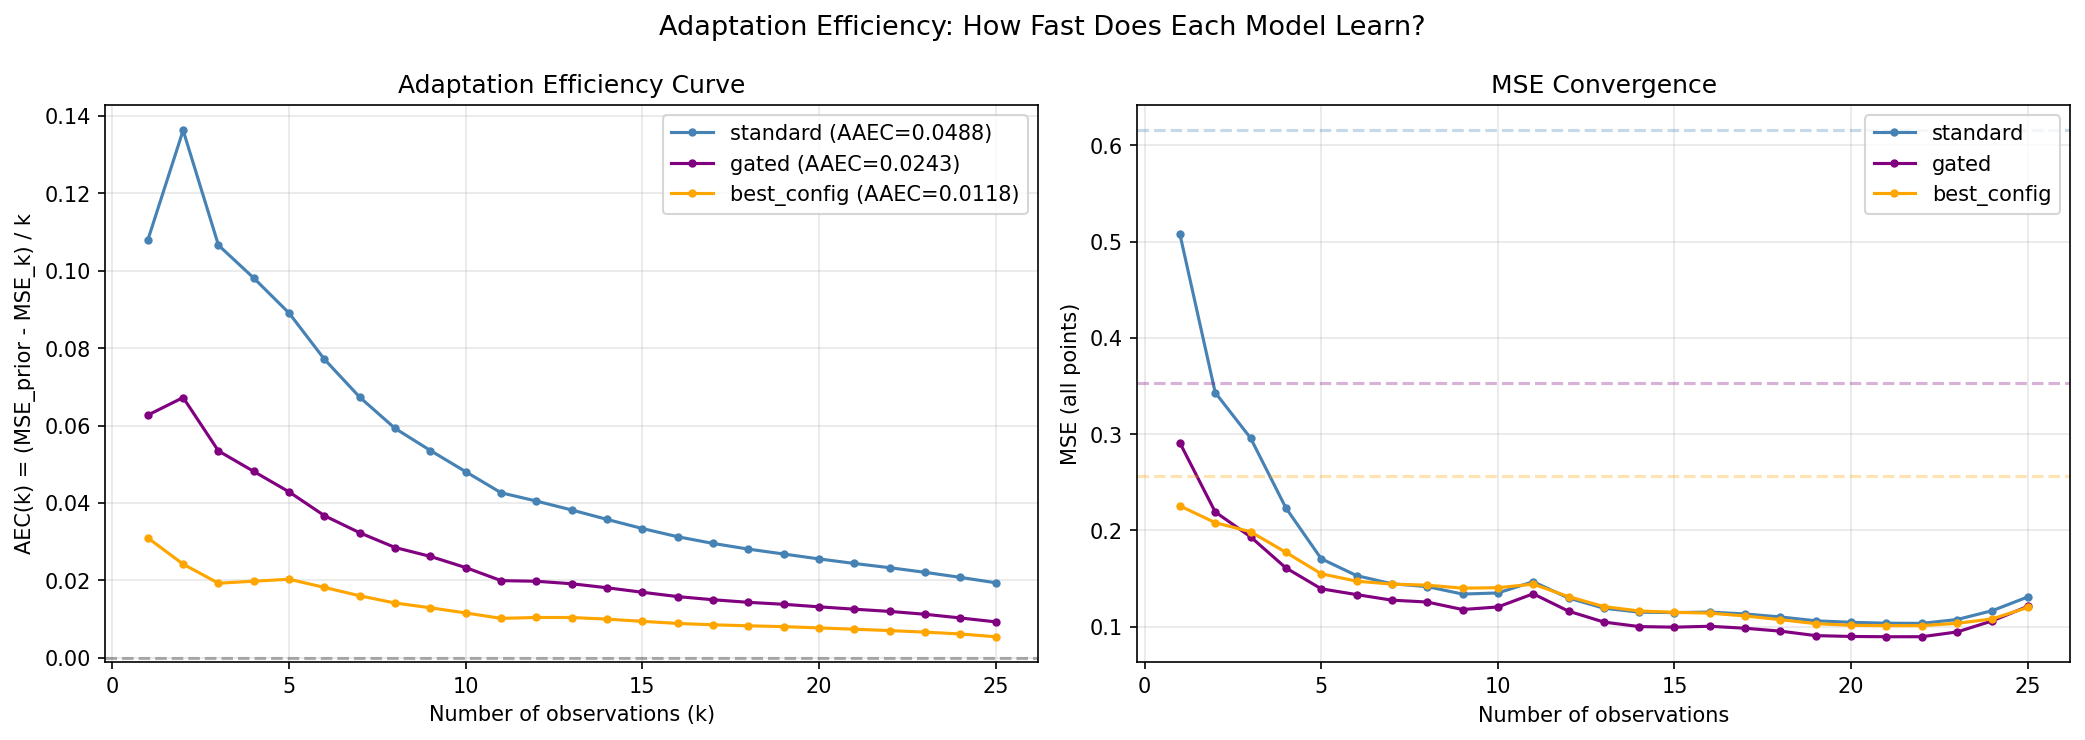
\includegraphics[width=\textwidth]{figures/aec_comparison.png}
    \caption{\textbf{Left:} Adaptation Efficiency Curves (AEC) for three model variants. The standard model has the highest per-observation efficiency because it starts from a higher prior MSE. \textbf{Right:} MSE convergence curves; dashed lines show prior MSE baselines.}
    \label{fig:aec}
\end{figure}

Figure~\ref{fig:aec} shows the Adaptation Efficiency Curves. The standard model achieves AAEC = 0.049 (highest per-observation efficiency) because it starts from a high prior MSE (0.616). The gated model's lower AAEC (0.024) reflects its already-accurate prior predictions (prior MSE = 0.354), there is less room to improve, which is itself a desirable property. The best-config model has the lowest AAEC (0.012) with a prior MSE of just 0.256.

\end{document}
